%================================================================
\section{Results and Discussion}\label{sec:Results}
%================================================================

%----------------------------------------------------------------
\subsection{Verifying the Implementation}\label{sec:project results}
%----------------------------------------------------------------

%----------------------------------------------------------------
\subsubsection{Non-Interacting}
%----------------------------------------------------------------

\autoref{fig:gridsearch} shows a VMC computations for a grid of $\alpha$ values for the non-interacting system for both the analytical and automatic differentiation approaches. 

\begin{figure}[H]
\centering
\subfloat[]{{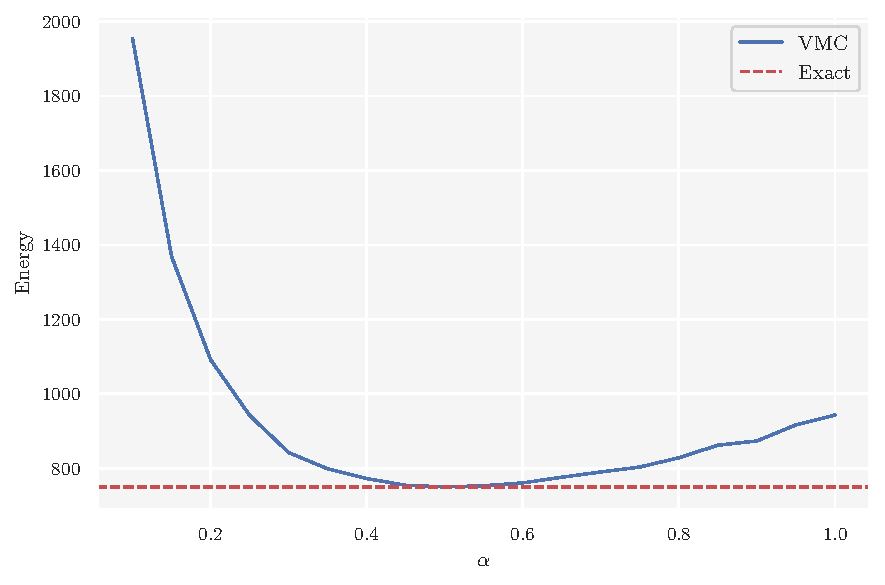
\includegraphics[scale=0.5]{latex/figures/grid_search_analytical.pdf}}}
\qquad
\subfloat[]{{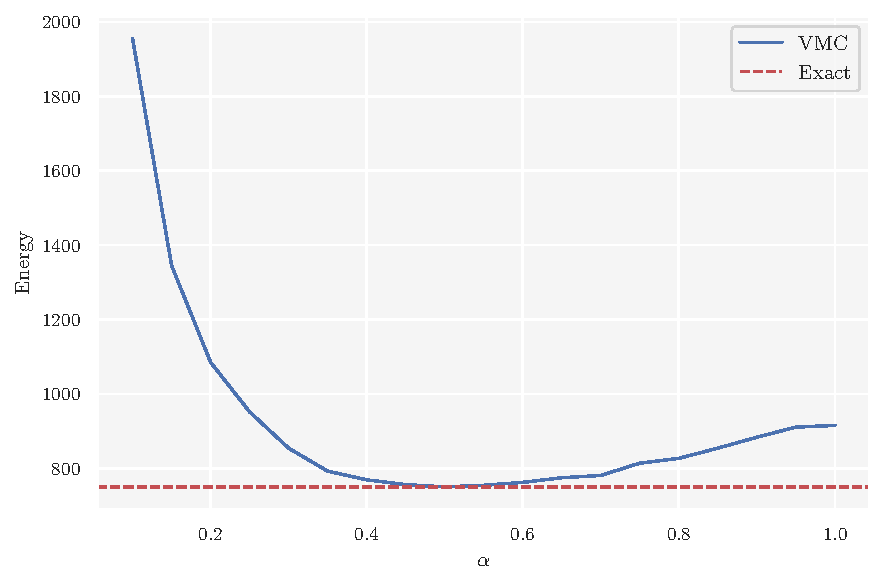
\includegraphics[scale=0.5]{latex/figures/grid_search_numerical.pdf}}}
\caption{Grid search $\alpha$, non-interacting system. \textbf{(a)} VMC computations with analytical expressions. \textbf{(b)} VMC computations with automatic differentiation.}
\label{fig:gridsearch}
\end{figure}



Discussion

%----------------------------------------------------------------
\subsubsection{Interacting}
%----------------------------------------------------------------

Compare log vs normal

%----------------------------------------------------------------
\subsection{Variational Energy}
%----------------------------------------------------------------

%----------------------------------------------------------------
\subsubsection{Non-Interacting}
%----------------------------------------------------------------

Discussion

\autoref{fig:non-interact_boxplot} shows 

\begin{figure}[!htb]
\centering
\subfloat[]{{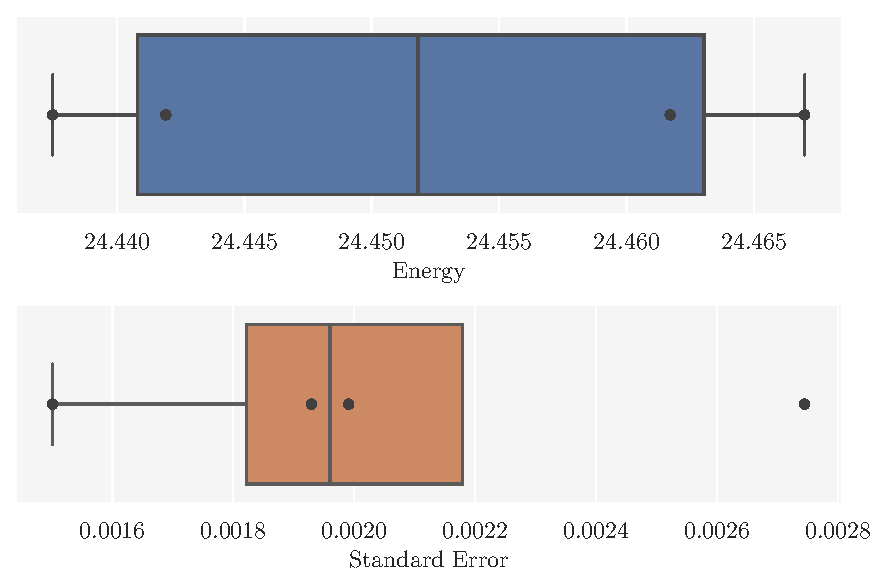
\includegraphics[scale=0.5]{latex/figures/boxplot_analytical_metropolis.pdf}}}
\qquad
\subfloat[]{{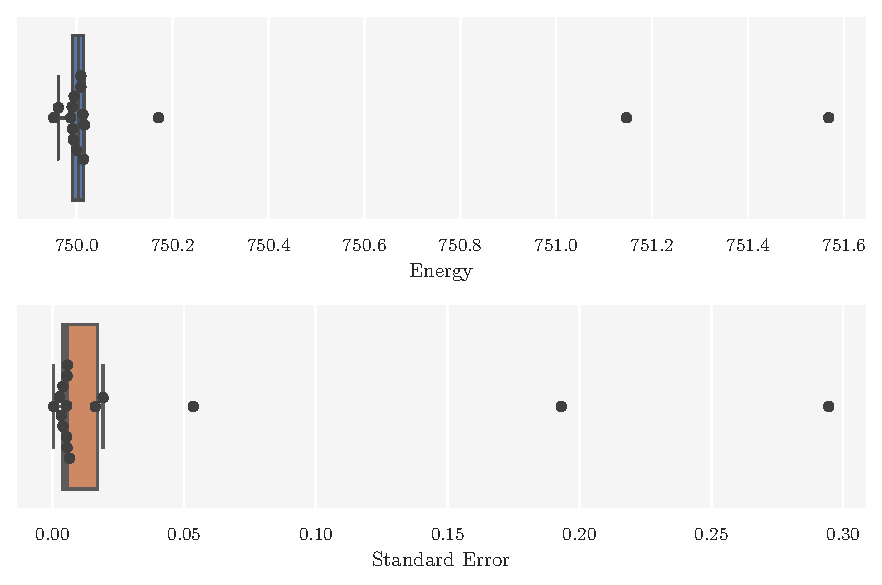
\includegraphics[scale=0.5]{latex/figures/boxplot_analytical_metropolis_hastings.pdf}}}
\qquad
\subfloat[]{{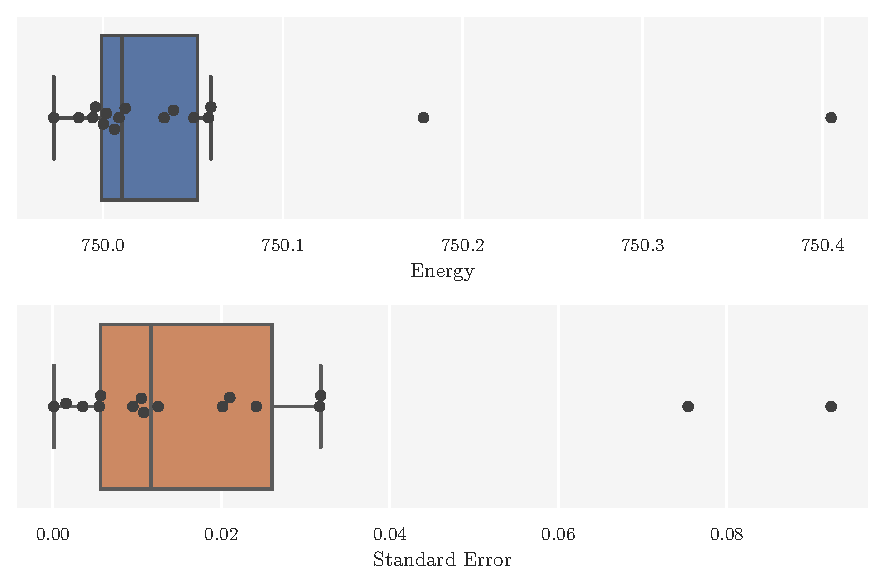
\includegraphics[scale=0.5]{latex/figures/boxplot_numerical_metropolis.pdf}}}
\qquad
\subfloat[]{{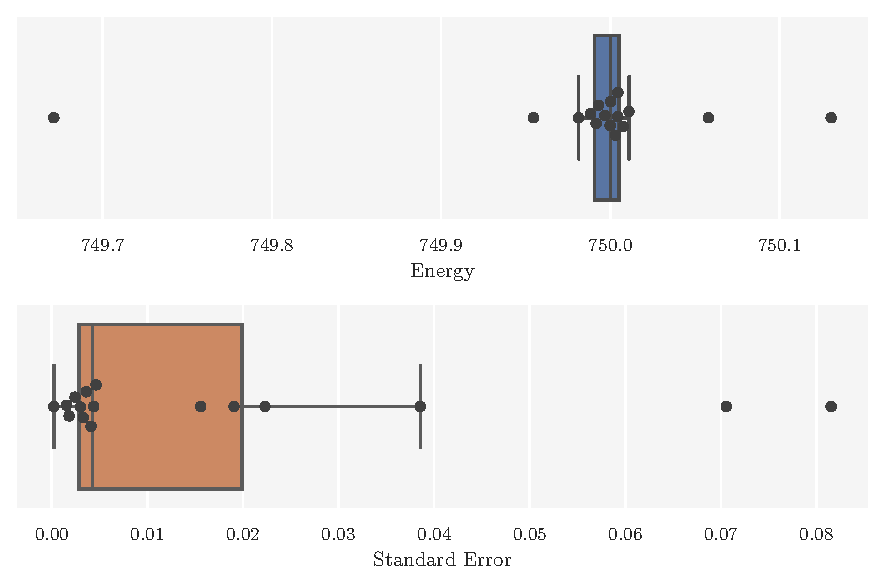
\includegraphics[scale=0.5]{latex/figures/boxplot_numerical_metropolis_hastings.pdf}}}
\caption{\textbf{(a)} Metropolis with analytical. \textbf{(b)} Metropolis-Hastings with analytical. \textbf{(c)} Metropolis with AD. \textbf{(d)} Metropolis-Hastings with AD.}
\label{fig:non-interact_boxplot}
\end{figure}

%----------------------------------------------------------------
\subsubsection{Interacting}
%----------------------------------------------------------------
\autoref{fig:interactions_plot} shows 
\begin{figure}[!htb]
\centering
\subfloat[]{{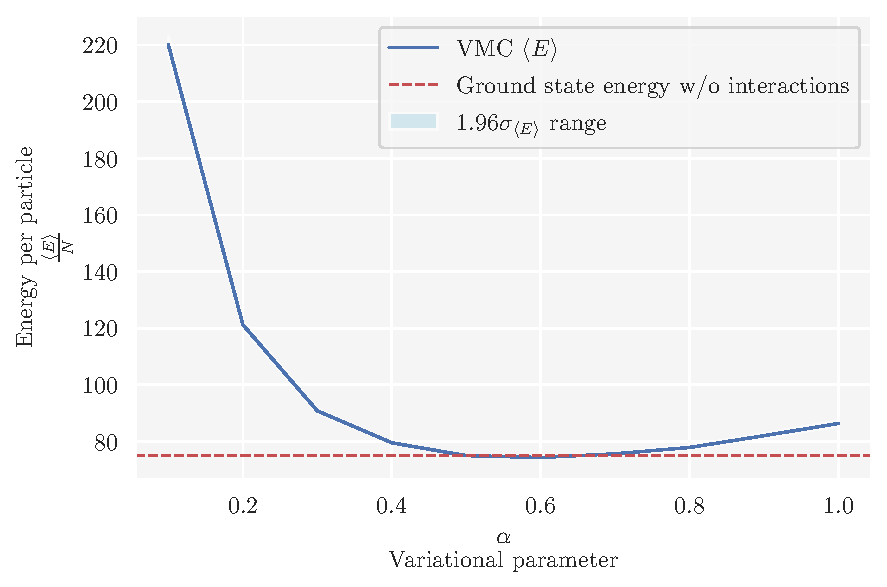
\includegraphics[scale=0.5]{latex/figures/grid_search_analytical_wo_interactions_N_50.pdf}}}
\qquad
\subfloat[]{{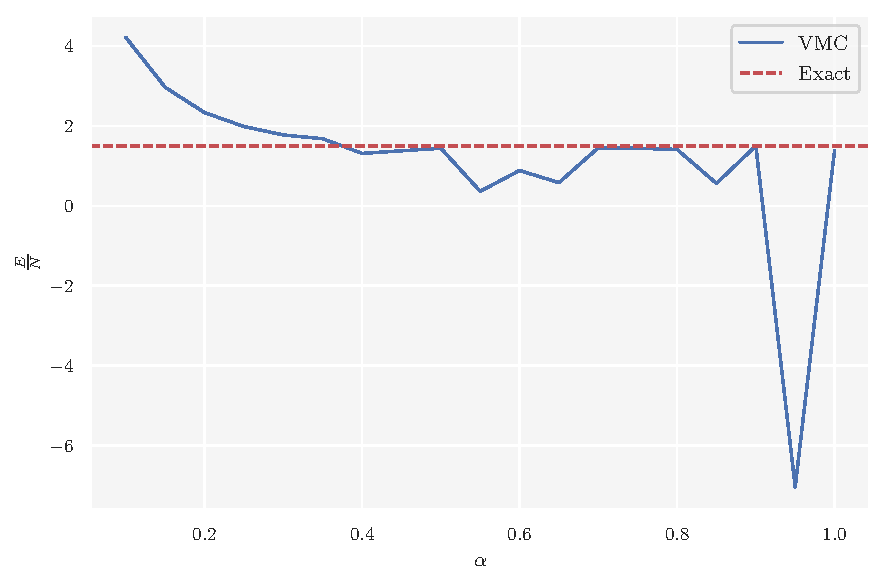
\includegraphics[scale=0.5]{latex/figures/grid_search_analytical_w_interactions_N_10.pdf}}}
\qquad
\subfloat[]{{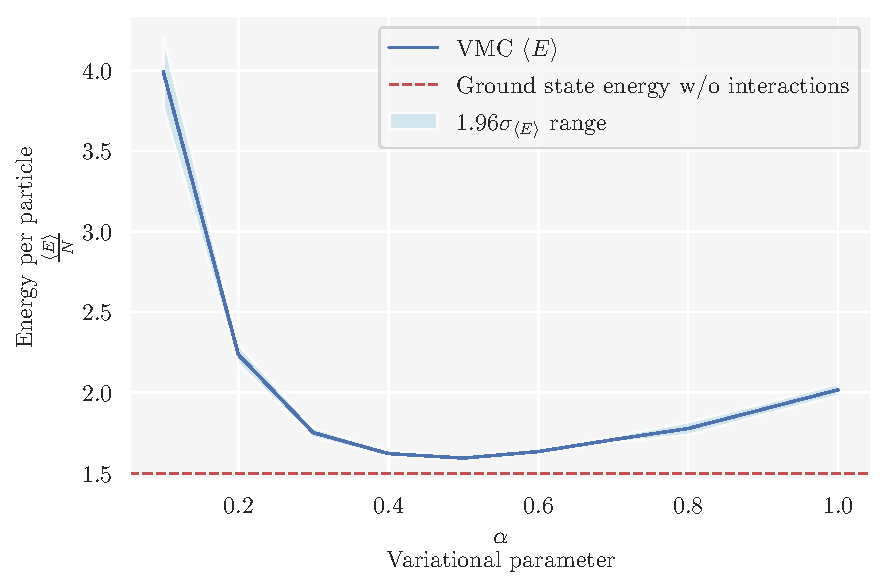
\includegraphics[scale=0.5]{latex/figures/grid_search_analytical_w_interactions_N_50.pdf}}}
\qquad
\subfloat[]{{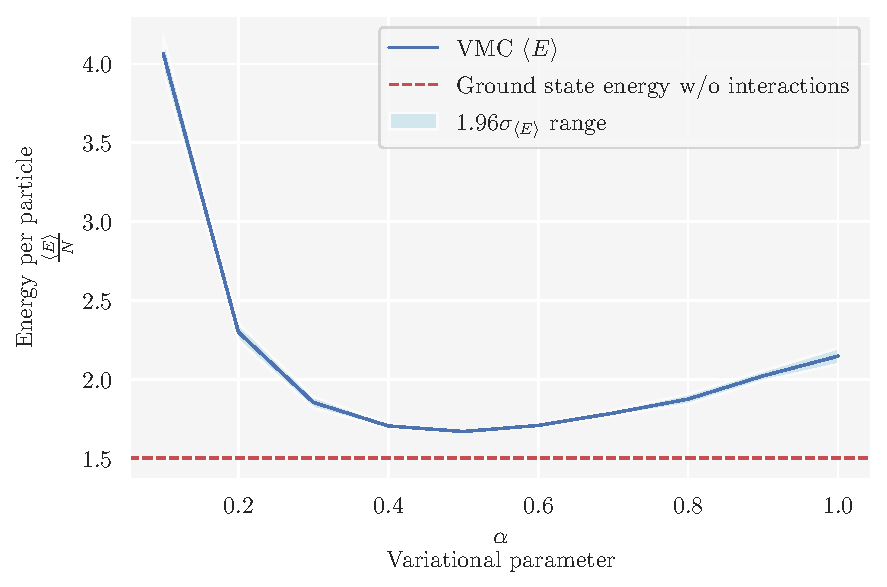
\includegraphics[scale=0.5]{latex/figures/grid_search_analytical_w_interactions_N_100.pdf}}}
\caption{\textbf{(a)} Metropolis with 50 non-interacting particles. \textbf{(b)} Metropolis with ten interacting particles. \textbf{(c)} Metropolis with 50 interacting particles. \textbf{(d)} Metropolis with 100 interacting particles.}
\label{fig:interactions_plot}
\end{figure}

\autoref{fig:comparisons_interactions_plot} shows 

\begin{figure}[H]
\begin{center}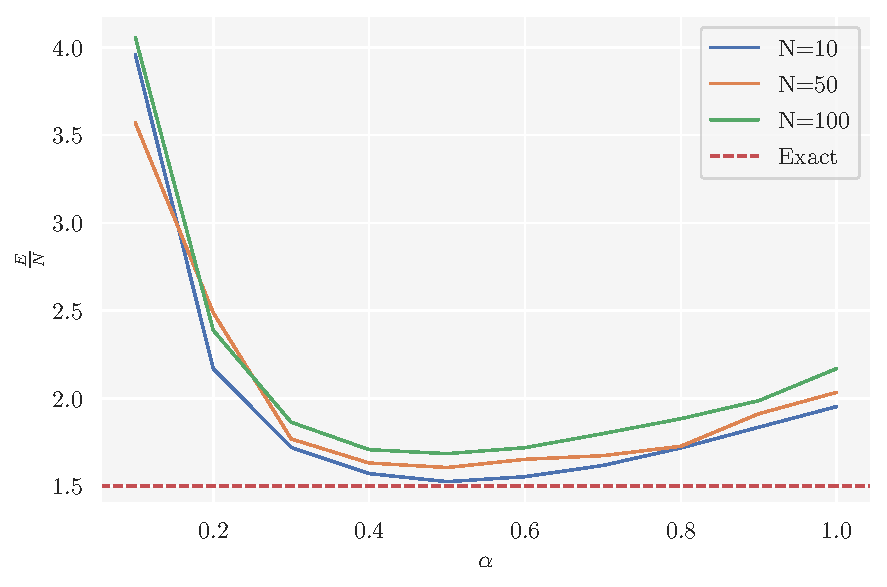
\includegraphics[scale=0.5]{latex/figures/grid_search_analytical_w_interactions_all_N.pdf}
\end{center}
\caption{Metropolis energy comparison between $N=10, 50, 100$ interacting particles, and $N=50$ non-interacting particles.}
\label{fig:comparisons_interactions_plot}
\end{figure}

\subsubsection{One-body densities}
\autoref{fig:one_body_densities} shows the sampled one body densities for $10$ and $100$ particles with interactions turned on and off. As the number of particles increases, the density of particles increases, and the interactions between the particles becomes a larger factor. For $10$ particles, the one body densities with and without interactions are almost identical. This means that for $10$ particles, the interactions do not have a large impact on the system. For $100$ particles, the radial one body densities for the interacting and non-interacting cases differ more. The particles in the interacting case are more spread out in the $2$-dimensional space than the non-interacting case. The interactions really do make a difference. 
\begin{figure}[H]
\centering
\subfloat[]{{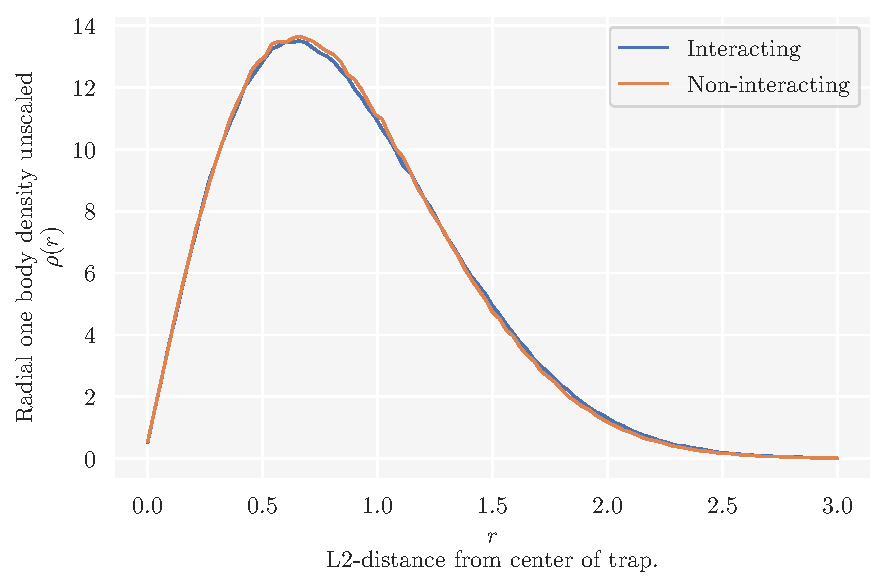
\includegraphics[scale=0.5]{latex/figures/OBD_N10.pdf}}}
\qquad
\subfloat[]{{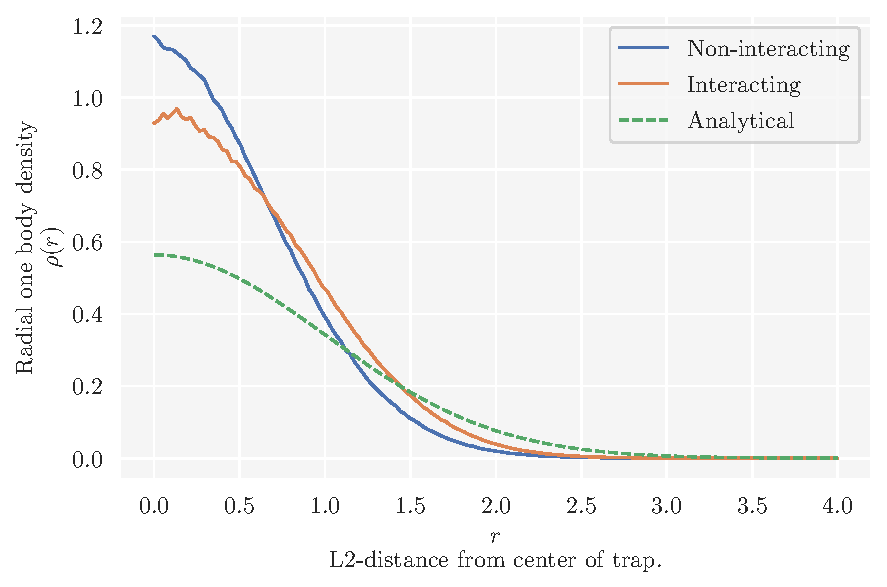
\includegraphics[scale=0.5]{latex/figures/OBD_N100.pdf}}}
\caption{\textbf{(a)} Comparison between the radial one body densities for $10$ particles with and without interactions (Jastrow factor $a=0.00433$) in $2$-dimensional space. \textbf{(b)} Comparison between the radial one body densities for $100$ particles with and without interactions (Jastrow factor $a=0.00433$) in $2$-dimensional space.}
\label{fig:one_body_densities}
\end{figure}